%%    _____  _____
%%   |  __ \|  __ \    AUTHOR: Pedro Rivero
%%   | |__) | |__) |   ---------------------------------
%%   |  ___/|  _  /    DATE: November 10, 2021
%%   | |    | | \ \    ---------------------------------
%%   |_|    |_|  \_\   https://github.com/pedrorrivero
%%

\section{Variational algorithms}

%% ----------------------------------------------------------------------------
%% ----------------------------------------------------------------------------

\begin{frame}[allowframebreaks]{Variational algorithms}

  One of the most promising near-term applications of quantum computers is the simulation of quantum mechanics. This is because:

  \begin{itemize}
    \item<2-> Quantum phenomena are exponentially hard to recreate by classical means, whilst thought to be efficiently reproducible using quantum resources: \textbf{quantum advantage}.
    \item<3-> This task is believed to be achievable in the foreseeable future thanks to \textbf{hybrid quantum-classical variational algorithms}.
    \item<4-> Promising applicability, especially for relatively low amounts of quantum resources: \textbf{Noisy Intermediate-Scale Quantum} era (NISQ).
  \end{itemize}

%% ----------------------------------------------------------------------------
\break
%% ----------------------------------------------------------------------------

  \begin{theorem}[Variational theorem]
    If the state $\ket{\psi}$ of a quantum system depends on some array of $n$ parameters $\qty{\theta^{n}}$, the optimal choice to approximate the ground state of said system (i.e. the eigenstate of its Hamiltonian $\hat{H}$ with minimum eigenvalue $\lambda_{\textnormal{min}}$) is the one which minimizes its Hamiltonian's expectation value $\ev*{\hat{H}}$. Assuming $\braket*{\psi}=1$:

    \begin{gather*}
      \ev{H}\!\qty(\theta^{n}) \equiv
        \ev{H}{\psi\qty(\theta^{n})} \geq
        \lambda_{\textnormal{min}} \, .
    \end{gather*}
  \end{theorem}

  Evaluating the expectation value of the different components making up our Hamiltonian is done through a process known as \textbf{operator averaging}:

  \begin{gather*}
    H_{N} = \sum_{j=1}^{\text{Poly}(N)} w_{j} P_{N}^{(j)} \qRa
    \ev{H_{N}} = \sum_{j=1}^{\text{Poly}(N)} w_{j} \ev{P_{N}^{(j)}}
  \end{gather*}

\end{frame}

%% ----------------------------------------------------------------------------
%% ----------------------------------------------------------------------------

\subsection{VQE and SSVQE}

%% ----------------------------------------------------------------------------
%% ----------------------------------------------------------------------------

\begin{frame}{Variational Quantum Eigensolver (VQE)}

	\begin{center}
		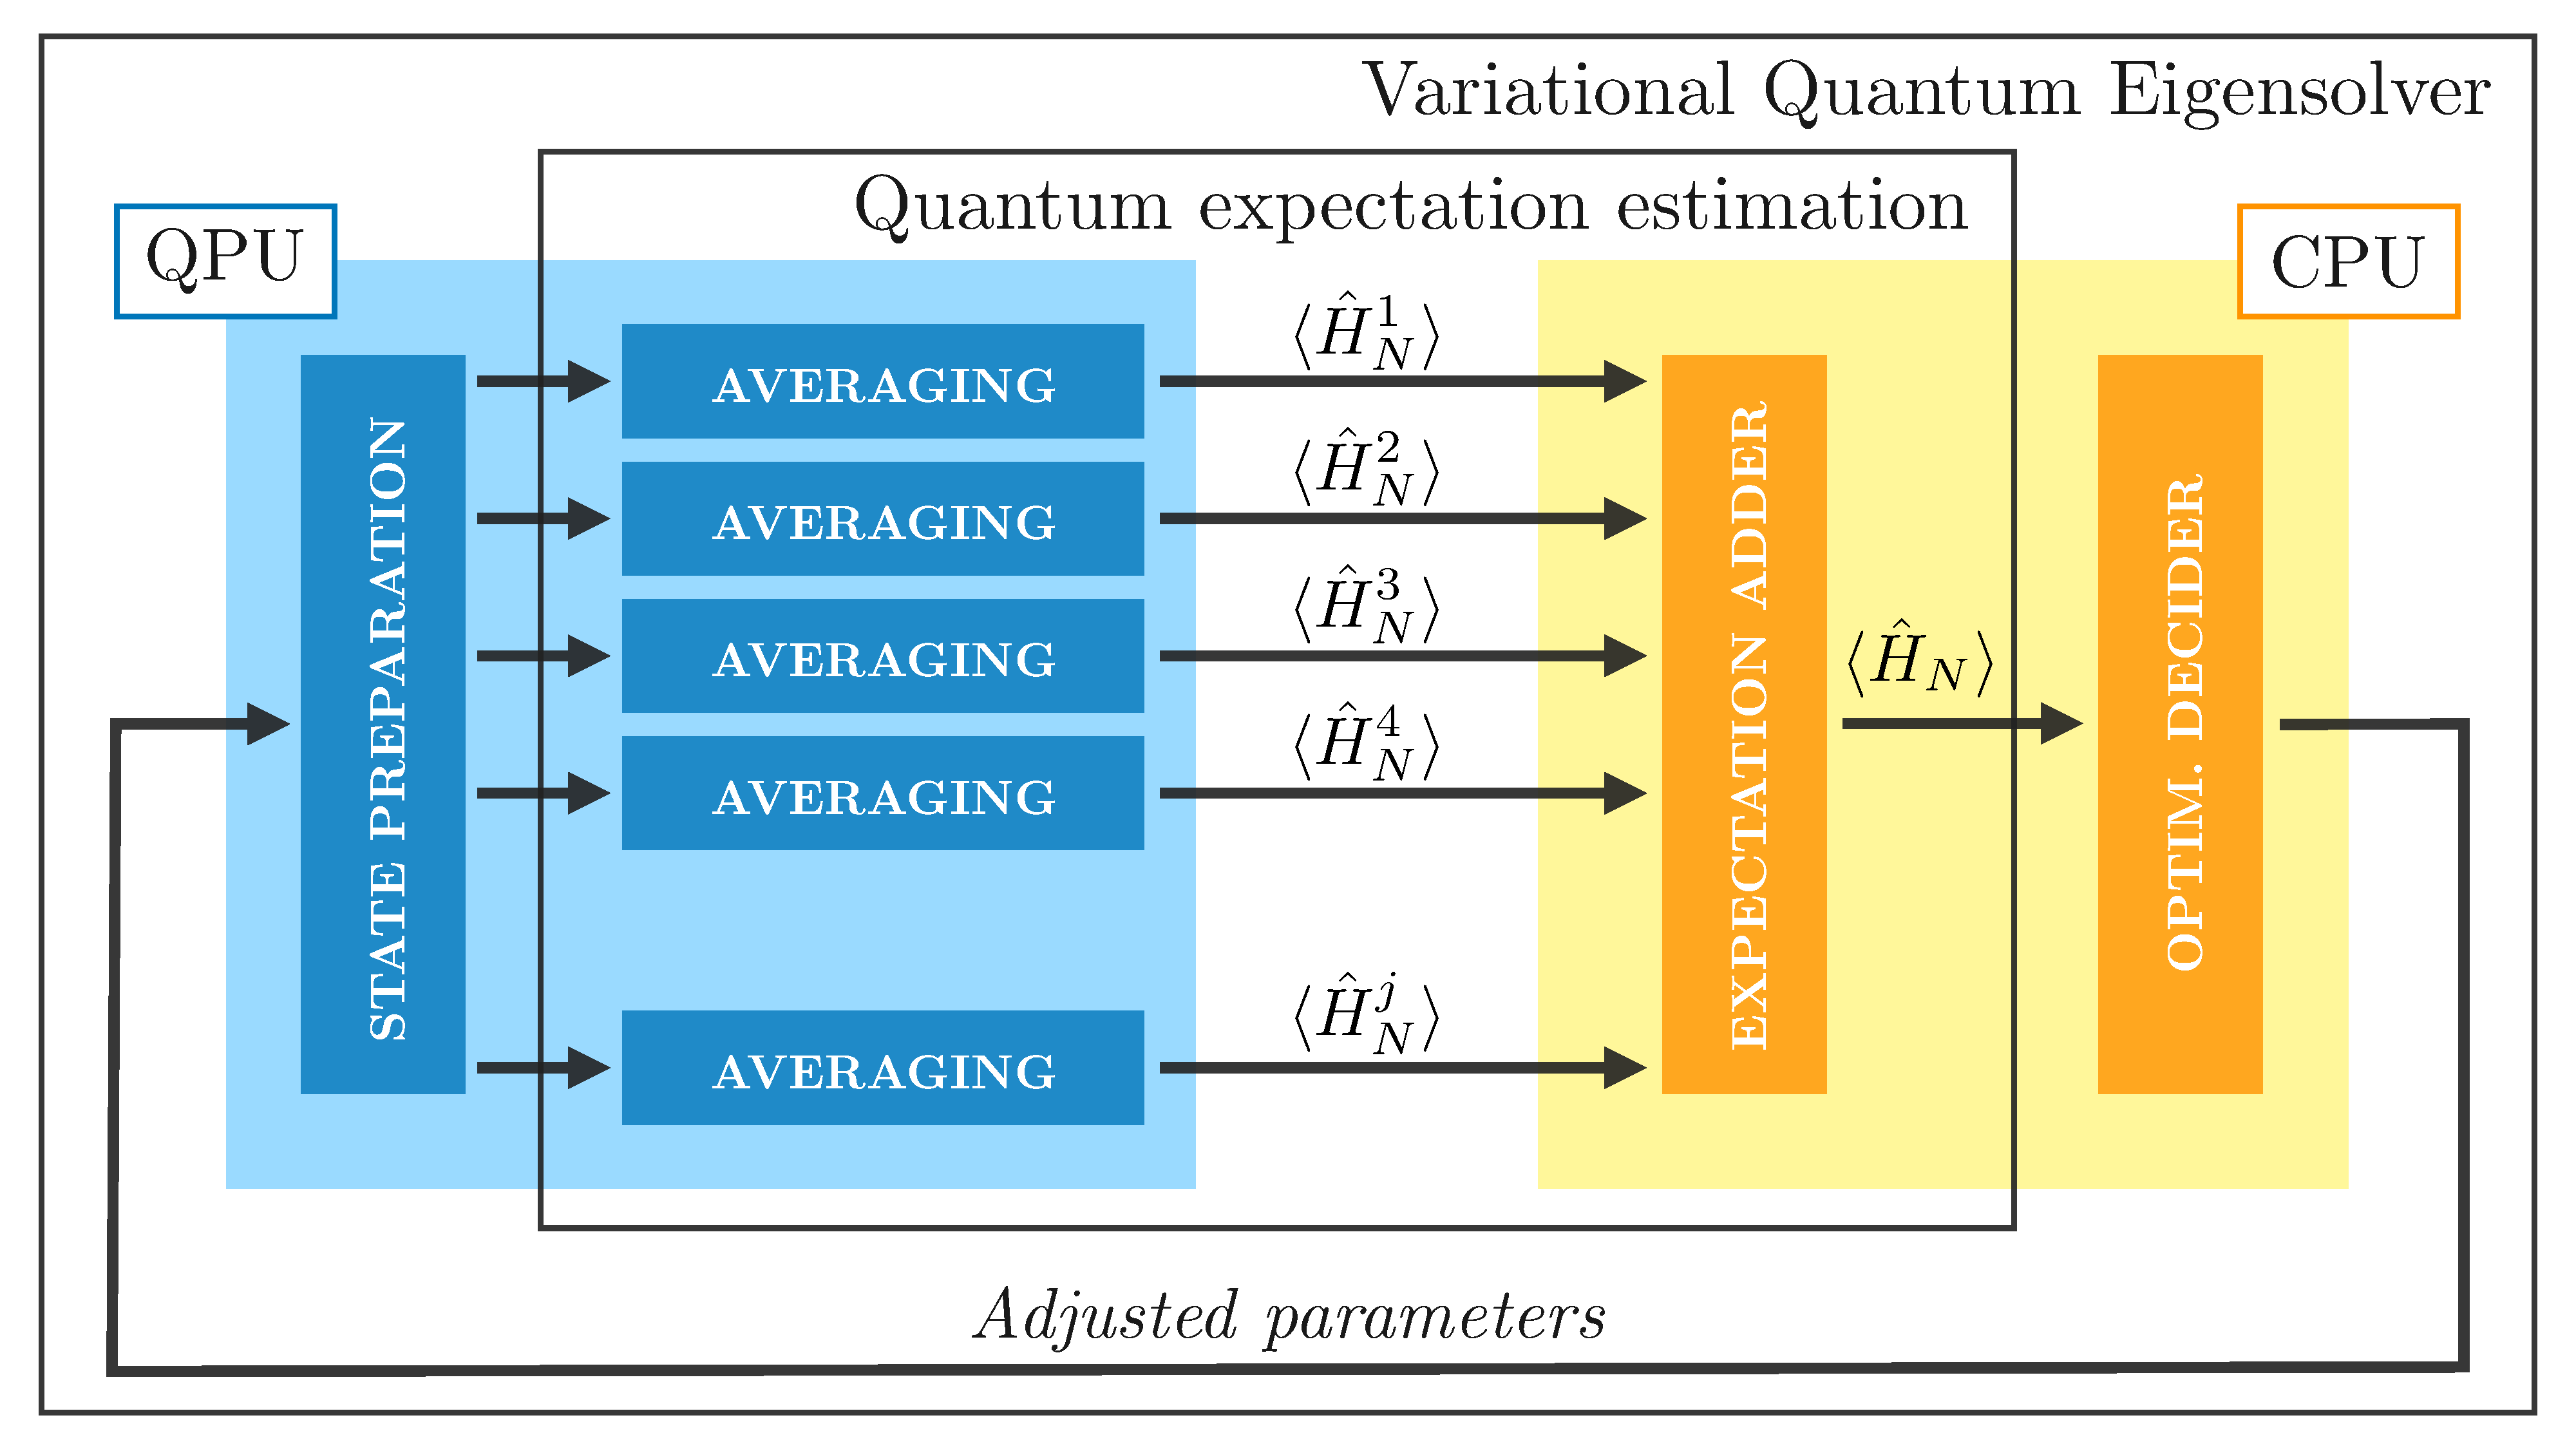
\includegraphics[width=.7\paperwidth]{Figures/chapter05/VQE}
	\end{center}

\end{frame}

%% ----------------------------------------------------------------------------
%% ----------------------------------------------------------------------------

\begin{frame}[allowframebreaks]{Subspace-search VQE (SSVQE)}

  Despite its success, VQE presents significant shortcomings that we would like to fix:

  \begin{itemize}
    \item<2-> Only prepare the minimum and maximum eigenstates of any given observable without having to modify it.
    \item<3-> Even if we were able to efficiently modify the observable to get other eigenstates, we would only be able to prepare one of those states at a time.
    \item<4-> Real-world problems require us to know not only the ground state, but also a number of relevant excited states.
  \end{itemize}

%% ----------------------------------------------------------------------------
\break
%% ----------------------------------------------------------------------------

  \textbf{Subspace-search VQE} can be summarized as:

  \begin{itemize}
    \item Construct an ansatz circuit $U(\theta)$ and choose input states $\qty{\ket{\varphi_j}}_{j=0}^{k}$ which are orthogonal with each other: $\braket{\varphi_i}{\varphi_j} =  \delta_{ij}$.
    \item Choose arbitrary weights so that $w_i > w_j$ if $i < j$, and minimize:
    \begin{gather*}
      \mathcal{L}_w(\theta) \defeq \sum_{j = 0}^{k} w_j \mel{\varphi_j}{U^\dagger(\theta) H U(\theta)}{\varphi_j} \qd
    \end{gather*}
  \end{itemize}

  Defining $\theta^*$ as the set of parameters that minimizes $\mathcal{L}_w(\theta)$, the ground state $\ket{\phi_{0}}$, and $k$ first excited states $\qty{\ket{\phi_{j}}}_{j=1}^k$ (in order) are approximated by:

  \begin{gather*}
    \ket{\phi_j} \cong U(\theta^*) \ket{\varphi_j} \qd
  \end{gather*}

  The catch with this algorithm is that it often requires a larger number of parameters and certain degree of redundancy in the way we prepare quantum states.

\end{frame}
